\chapter{Einleitung}

\section{Motivation}
\label{sec:Motivation}
\paragraph{}
Wenn man im Web nach einem Begriff sucht, kann die Suchanfrage nicht immer sofort genau definiert werden, besonders wenn das Thema der Suche dem Benutzer nicht bekannt ist. Um eine korrekte Anfrage aufbauen zu können, die die gewünschte Ergebnisse liefert, braucht man üblich mehr Iterationen - mit jeder Iteration wird die Anfrage präzisiert und verbessert. Da moderne Suchmaschinen allerdings keine strukturierte Informationen über die Suchergebnisse und auf der Suchergebnisseiten vorhandene Entitäten liefern, wird der Benutzer gezwungen, sich jedes Dokument manuell anzuschauen, um die Anregungen für neue Suchiterationen zu gewinnen, was als Folge zu einer niedrigen Arbeitsleistung führt.

Ein Beispiel für angesprochenes Problem ist auf der Abbildung \ref{fig:bing-issue} zu sehen. Man muss sich jeden gefundenen Snippet angucken und gelegentlich auch die gefundene Webseite öffnen, um die Antwort auf gestellte Frage zu erfahren, was bei längeren Sessionen viel Zeit in Anspruch nimmt.

\begin{figure}
\centering
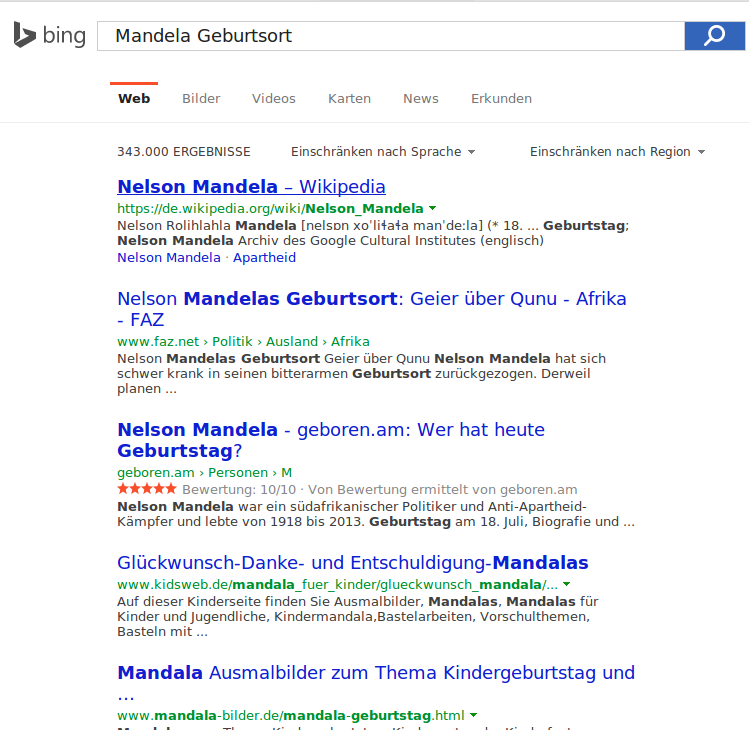
\includegraphics[width=1\textwidth]{Bilder/bing-search.png}
\caption{''Eine Websuche ohne Extraktion von Entitäten''}
\label{fig:bing-issue}
\end{figure}

Es existieren bereits mehrere Einsätze, die den Benutzer bei der Suche und bei der Präzision seiner Suchanfragen unterstützen und die die Websuche beschleunigen können:
\begin{itemize}
\item Personalisierung der Suche\cite{noll2007web} - es wird versucht, mithilfe von Suchhistorie des Benutzers, seines Verhaltens im Netz oder seinen ,,Likes``-Einträgen in sozialen Netzwerken die Ergebnisse, die für diesen Benutzer relevant wären, ,,vorherzusagen`` und den entsprechenden Dokumenten ein höheres Gewicht bei der Suche zu geben.
\item Automatische Vervollständigung der Anfrage - sobald man anfängt den Text der Anfrage zu tippen, werden dem Benutzer Vorschläge bezüglich des Restes der Anfrage gemacht.
\item Autokorrektur der Anfrage - falls es keine Dokumenten gefunden wurden, könnte die Anfrage bei Bedarf automatisch korrigiert werden.
\end{itemize}

In Rahmen dieser Arbeit soll ein anderer Einsatz implementiert und erforscht werden: die Extraktion von Entitäten aus Suchergebnissen. 

Eine Skizze der erwähntes Einsatzes ist auf der Abbildung \ref{fig:bing-and-entity} zu sehen. Die Idee dieses Einsatzes besteht daran, dass dem Benutzer zusätzlich zu den Links die Liste von sogenannten Entitäten - Personen, Firmen oder geographischen Objekten - angezeigt wird, die aus den Snippets (kurzen Textausschnitten der gefundenen Webseiten) extrahiert wurden. Der Einsatz könnte die Suche beschleunigen, da der Benutzer im besten Fall die verlinkte Dokumente gar nicht mehr öffnen muss, sondern sich lediglich die extrahierte Entitäten anschauen muss.

\begin{figure}
\centering
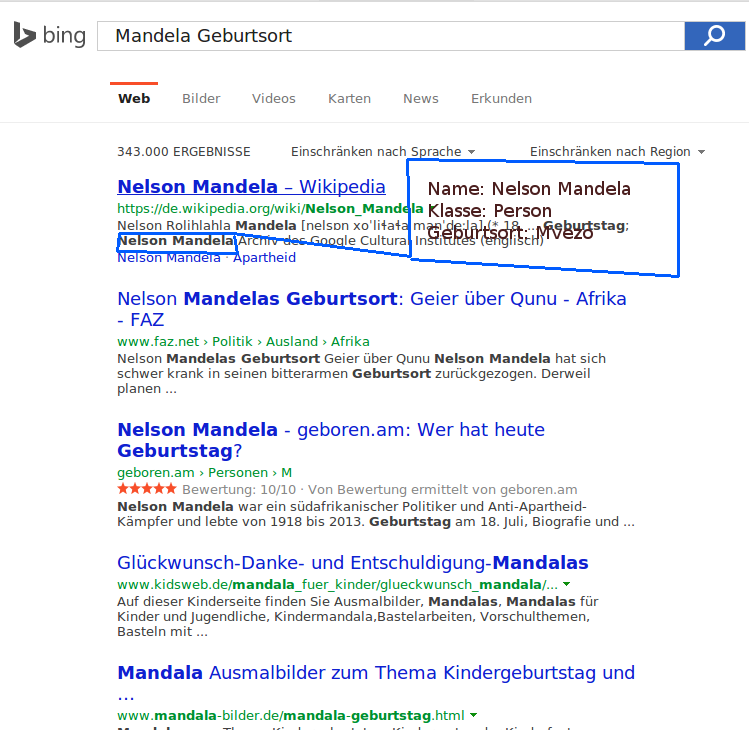
\includegraphics[width=1\textwidth]{Bilder/bing-and-entity.png}
\caption{''Eine Websuche mit Extraktion von Entitäten''}
\label{fig:bing-and-entity}
\end{figure}

Die Implementierung solches Einsatzes bringt mit sich allerdings bestimmte Herausforderungen, die im Rahmen dieser Arbeit angegangen werden müssen:

Erstens, es ist nicht klar, ob die kurze Textsnippets, die die Suchmaschinen liefern, für die Extraktion von Entitäten überhaupt benutzt werden müssen - das Problem ist, dass diese Textabschnitte sehr klein (üblicherweise zwei bis drei Sätze) sind, und es ist durchaus möglich, dass die gar keine Entitäten beinhalten.

Zweitens, der zusätzliche Schritt der Erkennung von Entitäten kann große Verzögerungen in die Suche bringen, was die Nutzbarkeit dieses Einsatzes zunichte machen könnte, wenn die Suche viel länger dauern wird, als die ohne der Extraktion von Entitäten.

Eine weitere Herausforderung wäre, dass jede natürliche Sprache ein besonderes an diese Sprache angepasstes Verfahren braucht, um erkennen zu können, welche Entitäten in dem Text vorkommen. Für englische Sprache existieren schon jetzt Verfahren und Modellen, mit deren Hilfe die englischsprachige Entitäten extrahiert werden können. Allerdings fehlt solches Modell für die deutsche Sprache, deswegen findet die Extraktion von deutschsprachigen Entitäten zurzeit nicht statt.

\paragraph{}
Eine reine Extraktion von Entitäten ist aber nicht ausreichend - der Extraktionischritt sagt nur, welche Tokens in dem Text möglicherweise eine Entität darstellen, die Informationen über die Entität - die dazugehörige Ontologien - fehlt nach dem Extraktionschritt noch. Um die entsprechende Ontologien mit den extrahierten Entitäten verlinken zu können, muss noch Entity Linking durchgeführt werden. Dafür wird für jede extrahierte Entität eine Suche in einer Wissendatenbank durchgeführt. Eine Wissendatenbank ist eine Datenbank, wo Ontologien für diverse Entitäten gespeichert werden. Für die Websuche kann DBpedia als Wissenbasis verwendet werden, allerdings für weniger generische Aufgaben, wie z.B. ein Suchsystem für Ärzte, wo der Suchdomain klar definiert ist, können andere Datenbanken verwendet werden.

\section{Aufgabenstellung}
\label{sec:Aufgabenstellung}
\paragraph{}
Die Arbeit umfasst drei große Abschnitte: 
\begin{itemize}
\item Zuerst soll ein Framework entwickelt werden, der die Extraktion und Verlinkung von Ontologien für deutschsprachige Webseiten ermöglicht. Die Webseiten werden dabei nicht im Plaintext ins System eingegeben, sondern als HTML. Deswegen soll der Framework auch rohe Textdaten aus dem HTML extrahieren können. 

\item Danach soll eine Bibliothek entwickelt werden, die dem Entwickler einfache API zur Anreicherung von Suchergebnissen zur Verfügung stellt. Der Entwickler soll idealerweise keine Wissen und Kenntnisse über Extraktion von Entitäten besitzen müssen.

\item Es soll anschließend eine Benutzerevaluierung durchgeführt werden, um feststellen zu können, ob man aus den Suchergebnissen gewonnene Entitäten für den Benutzer tatsächlich relevant sind.
\end{itemize}